%%http://users.stat.ufl.edu/~rrandles/sta4210/Rclassnotes/introduction-to-R/R-intro.pdf
%%%%%%%%%%%%%%%%%%%%%%%%%%%%%%%%%%%%%%%%%
% Beamer Presentation
% LaTeX Template
% Version 1.0 (10/11/12)
%
% This template has been downloaded from:
% http://www.LaTeXTemplates.com
%
% License:
% CC BY-NC-SA 3.0 (http://creativecommons.org/licenses/by-nc-sa/3.0/)
%
%%%%%%%%%%%%%%%%%%%%%%%%%%%%%%%%%%%%%%%%%
%----------------------------------------------------------------------------------------
%	PACKAGES AND THEMES
%----------------------------------------------------------------------------------------
\documentclass[aspectratio=169,serif,professionalfont]{beamer}
\mode<presentation> {
% The Beamer class comes with a number of default slide themes
% which change the colors and layouts of slides. Below this is a list
% of all the themes, uncomment each in turn to see what they look like.
%\usetheme{default}
%\usetheme{AnnArbor}
%\usetheme{Antibes}
%\usetheme{Bergen}
%\usetheme{Berkeley}
%\usetheme{Berlin}
% \usetheme{Boadilla}
% \usetheme{CambridgeUS}
%\usetheme{Copenhagen}
%\usetheme{Darmstadt}
% \usetheme{Dresden}
% \usetheme{Frankfurt}
%\usetheme{Goettingen}
%\usetheme{Hannover}
%\usetheme{Ilmenau}
%\usetheme{JuanLesPins}
%\usetheme{Luebeck}
\usetheme{Madrid}
%\usetheme{Malmoe}
% \usetheme{Marburg}
% \usetheme{Montpellier}
% \usetheme{PaloAlto}
% \usetheme{Pittsburgh}
% \usetheme{Rochester}
% \usetheme{Singapore}
%\usetheme{Szeged}
% \setheme{Warsaw}
% As well as themes, the Beamer class has a number of color themes
% for any slide theme. Uncomment each of these in turn to see how it
% changes the colors of your current slide theme.
\usepackage{color}
\usepackage{verbatim}
\usepackage{ragged2e}
\usepackage{courier}
\usepackage{graphicx}
\usepackage{amsfonts,multicol,multirow,float,colortbl}
\usepackage{fancybox}

}
\usepackage{verbatim}


\usepackage{graphicx,subfigure} % Allows including images
\usepackage{booktabs} % Allows the use of \toprule, \midrule and \bottomrule in tables
%\usepackage{pxfonts}
%\usepackage{eulervm}
\usepackage[T1]{fontenc} % Needed for Type1 Concrete
\usepackage{concrete,hyperref,csquotes,verbatim}
%\setbeamersize{text margin left=0.3in,text margin right=0.3in}

\title{Web App With Shiny}
\subtitle{(Shiny)}

%\titlegraphic{\includegraphics[height=2.5cm]{UWin.jpeg}}

\author{2113 Prachi Gore}
\institute[KBC NMU]{M.Sc.(Statistics) Department of Statistics\\School of Mathematical Sciences\\Kavayitri Bahinabai Chaudhari North Maharashtra University, Jalgaon}
\date{\today}
\setcounter{tocdepth}{3}
%\usepackage{ragged2e}
\apptocmd{\frame}{}{\justifying}{}
%\beamerdefaultoverlayspecification{<+->}
\setbeamercolor{block title}{fg=black,bg=gray!40}
\setbeamercolor{block body}{fg=black,bg=gray!10}
\setbeamercolor{block title alerted}{fg=red,bg=gray!40}
\setbeamercolor{block title example}{fg=black,bg=green!20}
\setbeamercolor{block body example}{fg=black,bg=green!5}
\setbeamerfont{block title}{series=\bfseries}

\newcommand{\abdf}[1]{}%{\begin{frame}[plain,c]{Assignment by: }\begin{center}\LARGE \textbf{#1}\end{center}\end{frame}}}

\usepackage{fourier}

\AtBeginSection[]{
    \begin{frame}
    \vfill
    \centering
    \begin{beamercolorbox}[sep=8pt,center,shadow=true,rounded=true]{title}
        \usebeamerfont{title}\insertsectionhead\par%
    \end{beamercolorbox}
    \vfill
    \end{frame}
}
%\newcommand{}\section{}{-}%\section}

\begin{document}

\begin{frame}
\maketitle
\end{frame}

\begin{frame}{Contents}
\begin{enumerate}
    \item \vspace{0.4cm}Introduction to Shiny
    \item \vspace{0.4cm}UserInterface
    \item \vspace{0.4cm}Introduction to Shiny
    \item \vspace{0.4cm}Server
    \item \vspace{0.4cm}What is ShinyDashboard
    \item \vspace{0.4cm}How to render Plot
    \item \vspace{0.4cm}References
\end{enumerate}
\end{frame}

\begin{frame}{Shiny}
\textbf{What is Shiny ?}\\ 
Shiny is an R package that makes it easy to build interactive web applications (apps) straight from R.\\ 
\textbf{How to install Shiny Package}\\
install.packages("shiny")\\
\textbf{How to use Shiny Package}\\
library("shiny")\\
\textbf{Structure of a Shiny App}\\
Shiny apps are contained in a single script called app.R\\
app.R has three components:\\
a user interface object\\
a server function\\
a shinyApp function\\
The user interface ui object controls the layout and appearance of our app. The server function contains the
instructions that our computer needs to build app. Finally the shinyApp function creates Shiny app from an
explicit UI/server pair.  
\end{frame}

%   \begin{frame}[fragile]
%   \textbf{ Let's Build a User Interface }
%   \frametitle{User Interface}
% \begin{verbatim}
% x <- c(1, 2, 3, 4, 5)
% mean(x)
% x=rnorm(100);
% a=function(x){
% return a;
% }

% \end{verbatim}
% \end{frame}

\begin{frame}[fragile]
  \textbf{ Let's Build a User Interface }
  \frametitle{User Interface}
\begin{verbatim}
library(shiny)
ui=fluidPage()
server=function(input,output){}
shinyApp(ui, server)
\end{verbatim}
\begin{figure}[htbp]
    \centering
    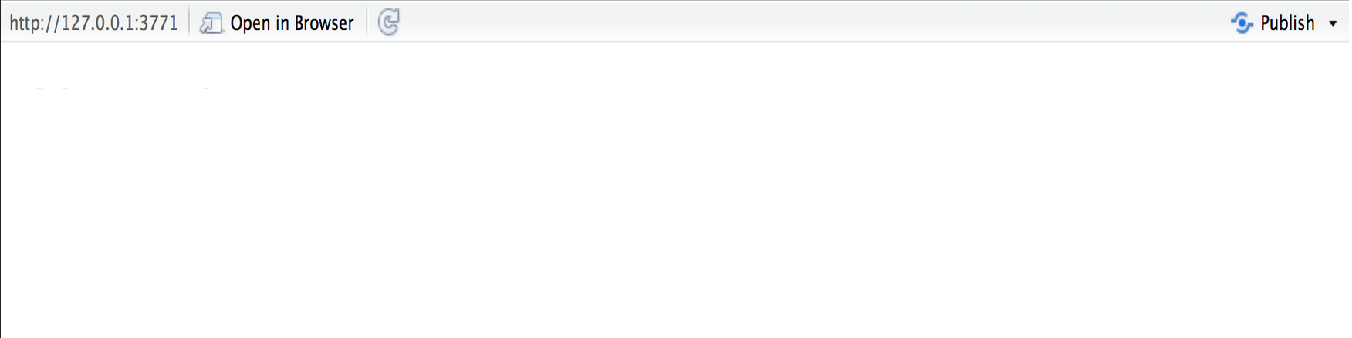
\includegraphics[width=0.8\textwidth]{blank_fluidpage.png}
    \caption{blank fluidpage}
    \label{fig:image_label1}
\end{figure}
\end{frame}

\begin{frame}[fragile]
 \frametitle{User Interface} 
\textbf{Layout}\\
Shiny uses the function fluidPage to create a display that automatically adjusts according to the\\ dimensions of user's browser window. we layout the user interface of our app by placing \\elements in the fluidPage function. \\For example, the ui function below creates a user interface \\that has a title panel and a sidebar layout , which includes a sidebar panel and a main panel. \\Note that these elements are placed within the fluidPage function.
\begin{verbatim}
ui = fluidPage(
    titlePanel("title panel"),
    sidebarLayout(
      sidebarPanel("sidebar panel"),
      mainPanel("main panel")
    )
  )            

\end{verbatim}
\end{frame}
\begin{frame}{User Interface}
    \begin{figure}[htbp]
    \centering
    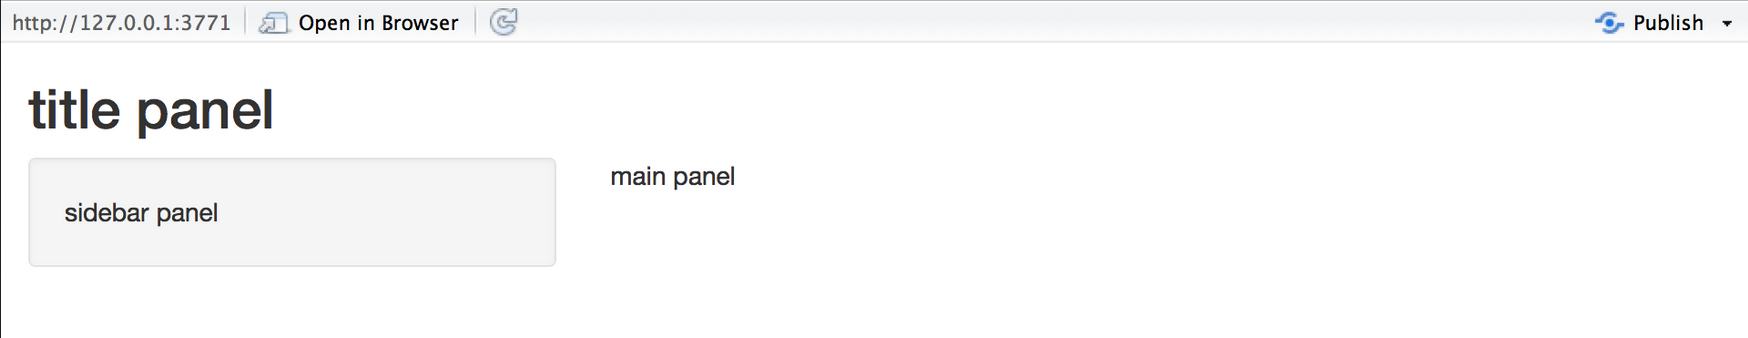
\includegraphics[width=0.8\textwidth]{fluidpage.png}
    \caption{fluidpage}
    \label{fig:image_label2}
\end{figure}
\end{frame}

\begin{frame}[fragile]
  \textbf{Display output }
  \frametitle{Server}
\begin{verbatim}
library(shiny)         
ui = fluidPage(
            titlePanel("title panel"),
            sidebarLayout(
                sidebarPanel("sidebar panel"),
                mainPanel(plotOutput('graph'))
                         )
                )
server=function(input,output){
                output$graph=renderPlot({hist(rnorm(100))})
               }
shinyApp(ui, server)                
\end{verbatim}
\end{frame}
\begin{frame}{Server}
\begin{figure}[htbp]
    \centering
    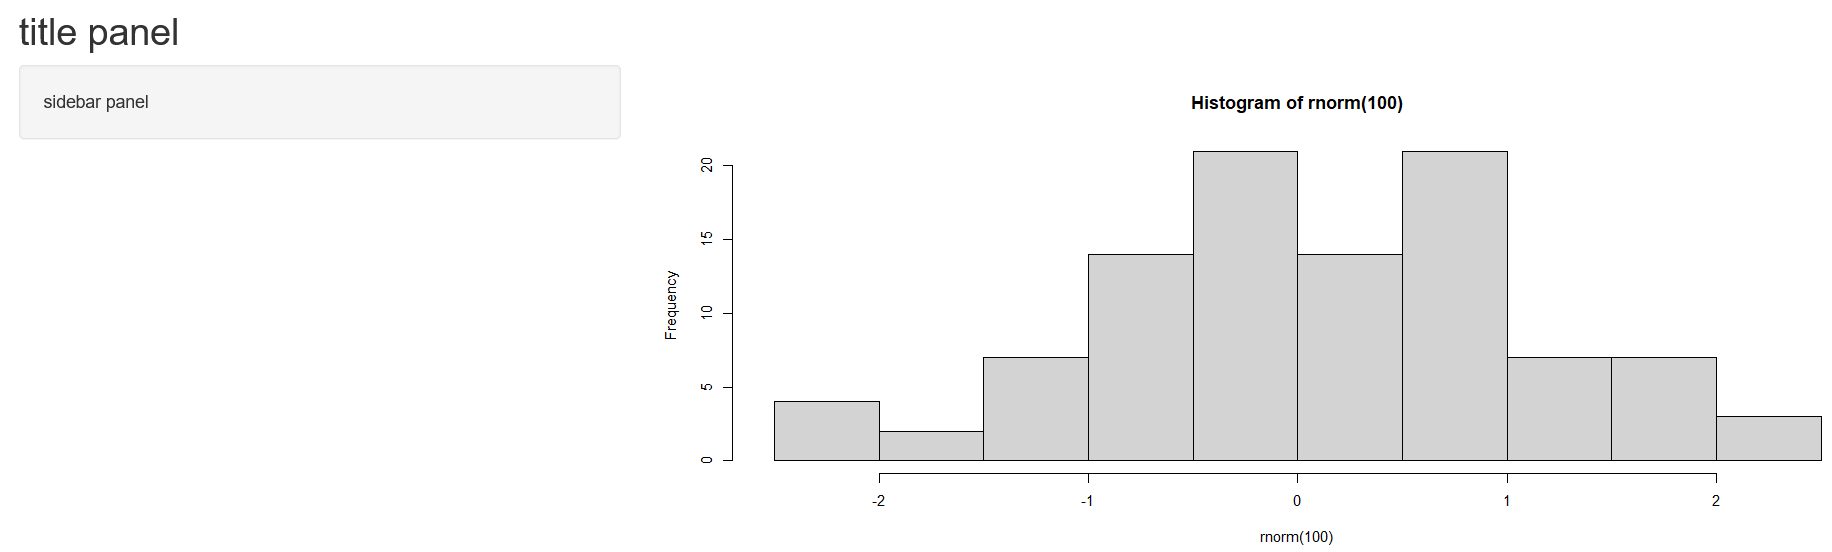
\includegraphics[width=0.8\textwidth]{histogram_output.png}
    \caption{histogram output}
    \label{fig:image_label3}
\end{figure}
\end{frame}

\begin{frame}[fragile]
  \textbf{Display reactive output}
  \frametitle{Server}
\begin{verbatim}
library(shiny)
ui = fluidPage(
     titlePanel("title panel"),
     sidebarLayout(
      sidebarPanel("sidebar panel",
                   numericInput(inputId = "n",label = "Enter Sample Size :",value = 50)),
      mainPanel(plotOutput('graph')))
             )
server=function(input,output){
    size= reactive({input$n})
    output$graph=renderPlot({hist(rnorm(size()))})
  }
shinyApp(ui, server)             
\end{verbatim}
\end{frame}
\begin{frame}{Server}
\begin{figure}[htbp]
    \centering
    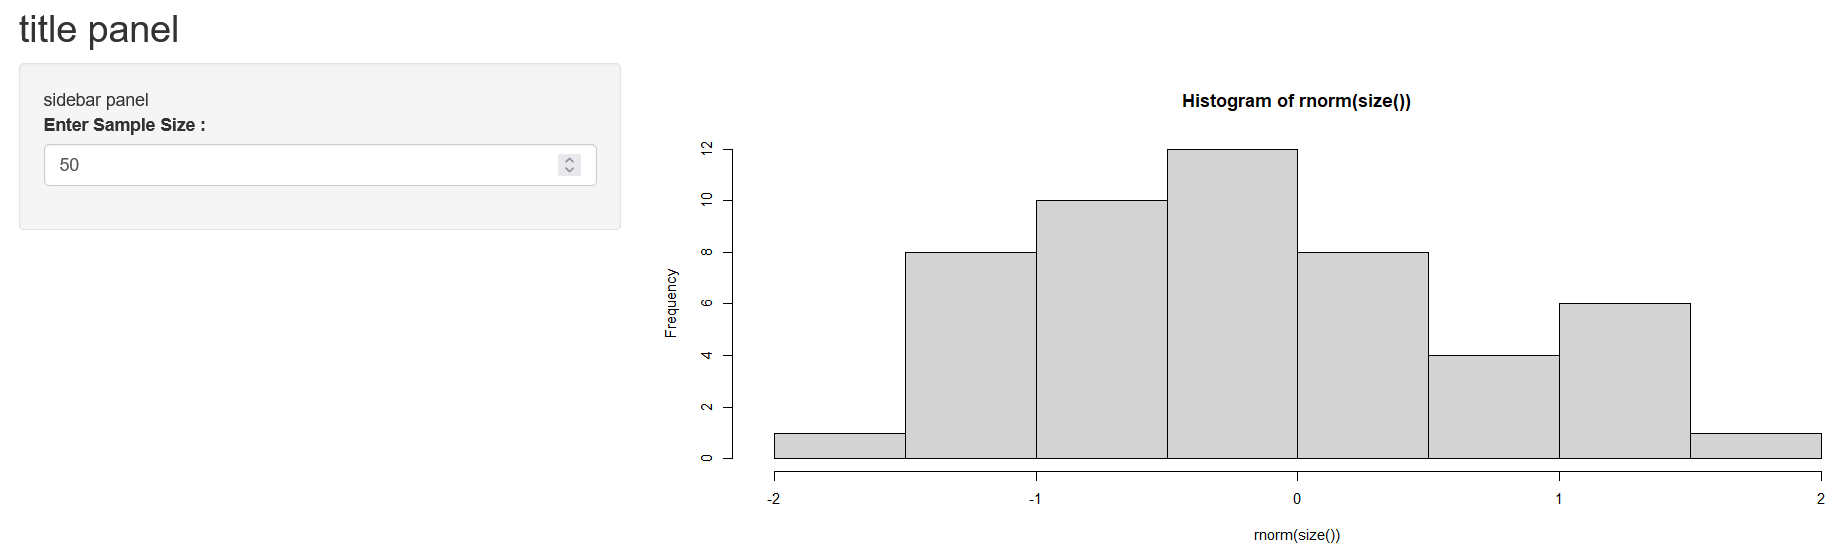
\includegraphics[width=0.8\textwidth]{reactive_output.png}
    \caption{reactive output}
    \label{fig:image_label4}
\end{figure}
here histogram is depend on sample size and sample size is in user's hand it could be anything 10,30,100,500,...so we will write it in reactive({}) function Whenever User update the sample size plot will be re render. Now this time entire file will not run again Whenever changes happens only that part will be run again. this is the power of reactive function and it help to improve speed of app.
\end{frame}

\begin{frame}[fragile]
  \frametitle{Shiny Dashboard}
  \textbf{Installation}\\
install.packages("shinydashboard")\\
\textbf{Layout}\\
A dashboard has three parts. a dashboardHeader( ) , a dashboardSidebar( ) and a dashboardBody( ) .\\
\begin{verbatim}
library(shiny)
library(shinydashboard)
ui = dashboardPage(
dashboardHeader(),
dashboardSidebar(),
dashboardBody()
)
server = function(input, output) { }
shinyApp(ui, server)    
\end{verbatim}
\end{frame}

\begin{frame}{Shiny Dashboard}
    \begin{figure}[htbp]
    \centering
    
\includegraphics[width=0.8\textwidth,height=4cm]{blank_dashboard.png}
    \caption{blank dashboard}
    \label{fig:image_label5}
   \end{figure}
   \begin{figure}[htbp]
    \centering
    
\includegraphics[width=0.8\textwidth,height=1cm]{header.png}
    \caption{header}
    \label{fig:image_label6}
   \end{figure}
\end{frame}

\begin{frame}[fragile]
  \frametitle{Shiny Dashboard}
  \textbf{Header}\\
\begin{verbatim}
library(shiny)
 library(shinydashboard)
 ui = dashboardPage(
 dashboardHeader(title = "Web App",
 tags$li(class="dropdown",tags$a(href="https://github.com/Prachi-Gore",
 icon("github"),target="_blank")),
 tags$li(class="dropdown",tags$a(href="https://www.linkedin.com/in/prachi-gore-4772a11a5",
 icon("linkedin"),target="_blank"))),
 dashboardSidebar(),
 dashboardBody()
 )
 server = function(input, output) { }
 shinyApp(ui, server)   
\end{verbatim}
\end{frame}

\begin{frame}[fragile]
  \frametitle{Shiny Dashboard}
  \textbf{Sidebar}\\
\begin{verbatim}
library(shiny)
library(shinydashboard)
ui = dashboardPage(
dashboardHeader(),
dashboardSidebar(
sidebarMenu(
id = "tabs",menuItem("Graph", tabName = "graph",menuSubItem("Scatter Plot", tabName = "Scatter-                                                 Plot"),menuSubItem("Box Plot", tabName = "Box-Plot"))
)),
dashboardBody()
)
server = function(input, output) { }
shinyApp(ui, server) 
\end{verbatim}
\end{frame}

\begin{frame}{Shiny Dashboard}
    \begin{figure}[htbp]
    \centering
    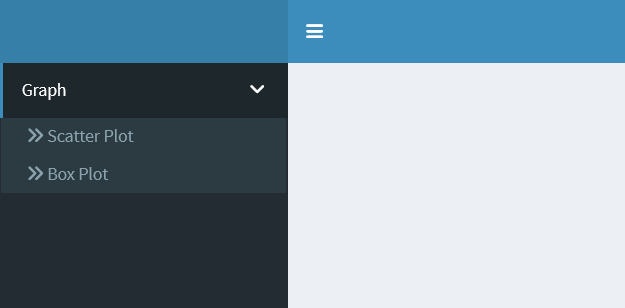
\includegraphics[width=0.8\textwidth,height=2cm]{sidebar.png}
    \caption{blank dashboard}
    \label{fig:image_label7}
   \end{figure}
   \begin{figure}[htbp]
    \centering
    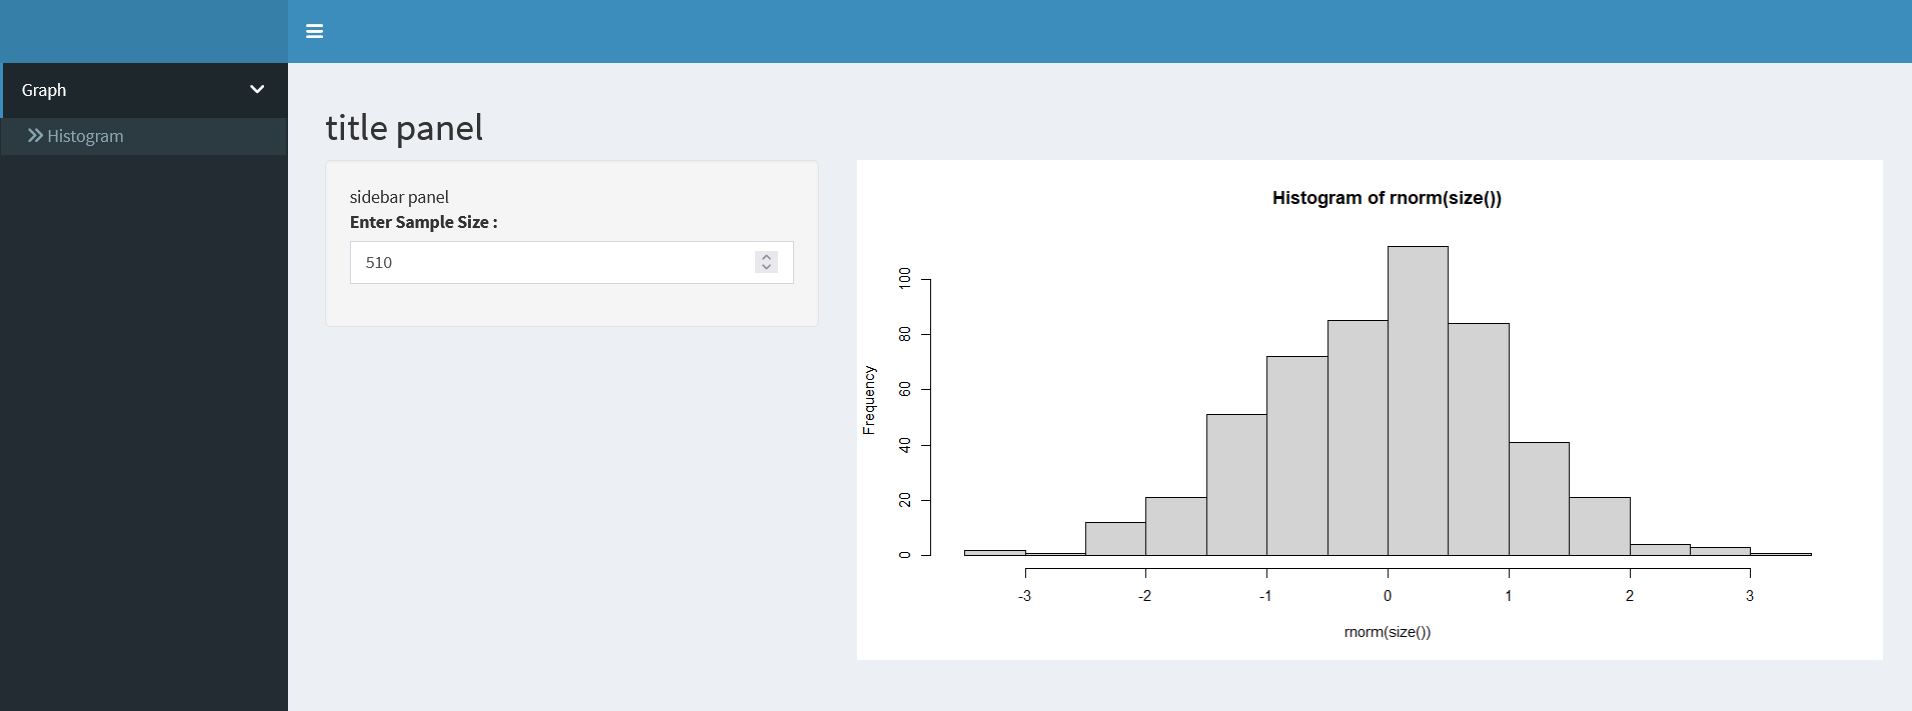
\includegraphics[width=0.8\textwidth,height=3cm]{body.png}
    \caption{header}
    \label{fig:image_label8}
   \end{figure}
\end{frame}

\begin{frame}[fragile]
  \frametitle{Shiny Dashboard}
  \textbf{Body}\\
\begin{verbatim}
 library(shiny)
 library(shinydashboard)
 ui_hist = fluidPage(
 titlePanel("title panel"),
 sidebarLayout(
 sidebarPanel("sidebar panel",
 numericInput(inputId = "n",label = "Enter Sample Size :",
 value = 50)),
 mainPanel(plotOutput("histogram"))
 )
 )
 
\end{verbatim}
\end{frame}

\begin{frame}[fragile]
  \frametitle{Shiny Dashboard}
\begin{verbatim}
 ui = dashboardPage(
 title="dashboard page",
 dashboardHeader(),
 dashboardSidebar(
 sidebarMenu(
 id = "tabs",
 menuItem("Graph", tabName = "graph",
 menuSubItem("Histogram", tabName = "histogram"))
           )
           ),
 dashboardBody(tabItems(tabItem(tabName = "histogram",ui_hist)))
 )  
\end{verbatim}
\end{frame}

\begin{frame}[fragile]
  \frametitle{Shiny Dashboard}
\begin{verbatim}
 server=function(input,output){
 size= reactive({input$n})
 output$histogram=renderPlot({hist(rnorm(size()))})
 }
 shinyApp(ui, server) 
 \end{verbatim}
 \begin{figure}[htbp]
    \centering
    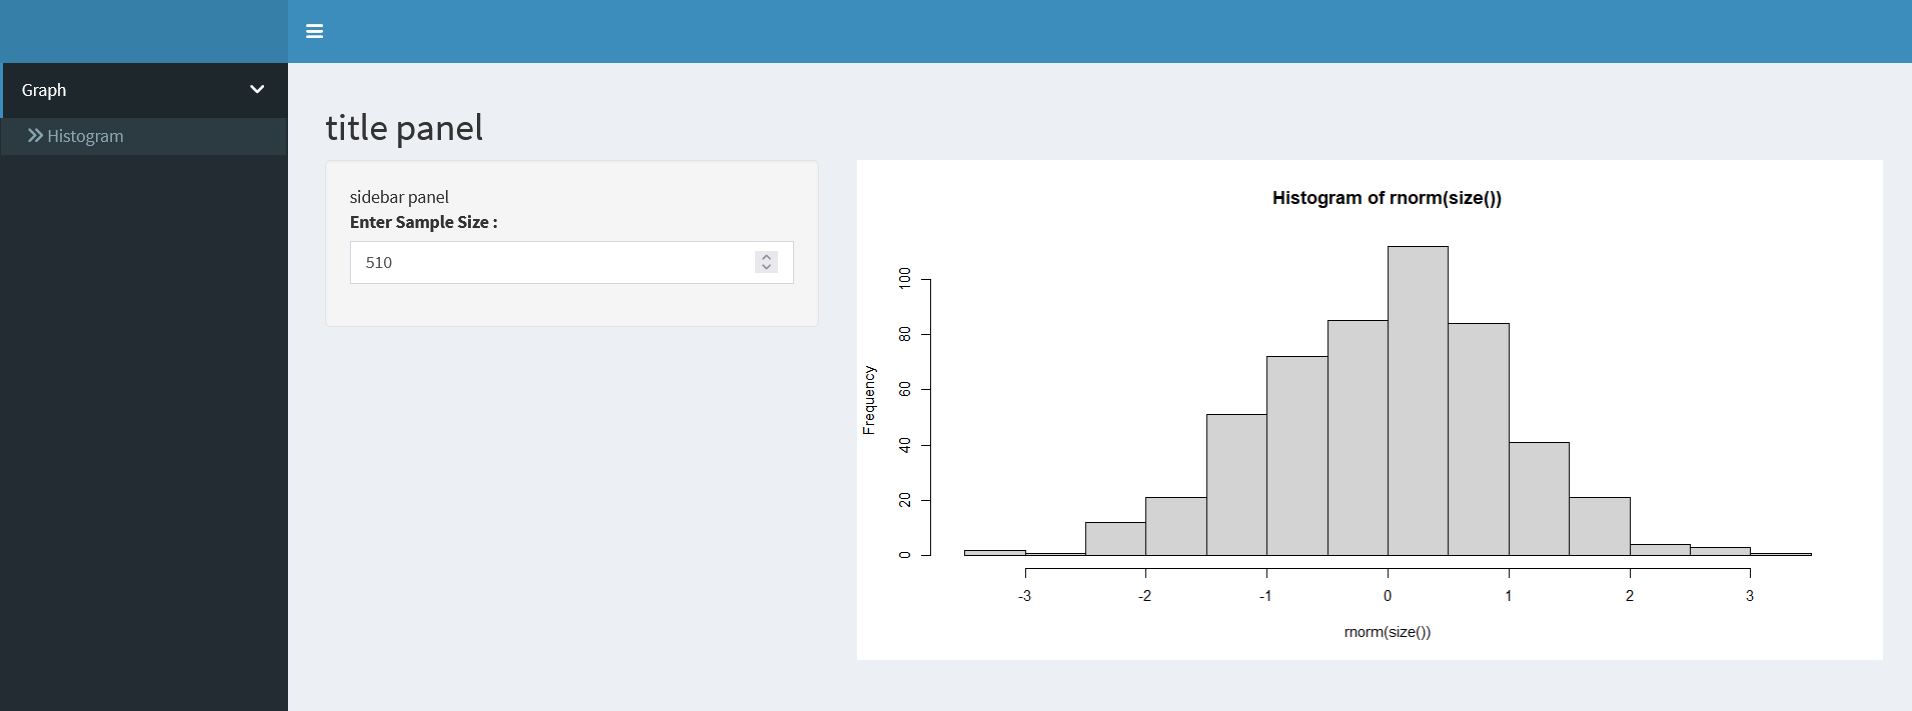
\includegraphics[width=0.8\textwidth,height=3cm]{body.png}
    \caption{ dashboard body}
    \label{fig:image_label9}
   \end{figure}

\end{frame}


\begin{frame}[fragile]
  \frametitle{How to render Scatter Plot}
\begin{verbatim}
 library(shiny)
 library(shinydashboard)
 library(tools) #to check file extension
 library(dplyr) #select_if()
 library(readxl)
 scatter_ui=fluidPage(title="scatter",sidebarLayout(sidebarPanel(
 fileInput(inputId = "file_scatter", label = "Select Dataset",
 accept = c(".csv",".xlsx"),
 buttonLabel = "Browse...",placeholder = "No file selected"),
 selectInput(inputId = "scatter_var1_id",
 label = "Select x variable",choices=""),
 selectInput(inputId = "scatter_var2_id",
 label = "Select y variable",choices="")),
 mainPanel (plotOutput("scatter")) ))
\end{verbatim}
\end{frame}

\begin{frame}[fragile]
  \frametitle{How to render Scatter Plot}
\begin{verbatim}
 header = dashboardHeader()
 sidebar=dashboardSidebar(sidebarMenu(id = "tabs",
                menuItem("Graph", tabName = "graph",
                menuSubItem("Scatter Plot", tabName = "Scatter-Plot"))))
 body=dashboardBody(tabItems(tabItem("Scatter-Plot",scatter_ui)))
 ui = dashboardPage(title ="Web App With Shiny",header,sidebar,body)
 update_input= function(input_id,label,data){return(
 updateSelectInput(
 session = getDefaultReactiveDomain(),
 inputId = input_id,
 label = label,
 choices = names(data()),
 selected = NULL))
 }
 
\end{verbatim}
\end{frame}

\begin{frame}[fragile]
  \frametitle{How to render Scatter Plot}
\begin{verbatim}
 server= function(input,output){
 data_scatter=reactive({
 req(input$file_scatter)
 file_ext= file_ext(input$file_scatter$datapath)
 if(file_ext=="xlsx"|file_ext=="xls"){
 df=as.data.frame(read_excel(input$file_scatter$datapath))}
 else{df = read.csv(input$file_scatter$datapath )}
 return(select_if(df, is.numeric))
 })

\end{verbatim}
\end{frame}

\begin{frame}[fragile]
  \frametitle{How to render Scatter Plot}
\begin{verbatim}
 observe(update_input("scatter_var1_id",label="select X variable",
                      data_scatter))
 observe(update_input("scatter_var2_id",label="select Y variable",
                       data_scatter))
 output$scatter = renderPlot({
 x = data_scatter()[,input$scatter_var1_id]
 y=data_scatter()[,input$scatter_var2_id]
 plot(x,y,xlab=input$scatter_var1_id,ylab=input$scatter_var2_id,
 main = paste("Scatter plot of" ,input$scatter_var1_id,"vs",
 input$scatter_var2_id))
 })
 }
 shinyApp(ui,server)
\end{verbatim}
\end{frame}

\begin{frame}{How to render Scatter Plot}
   \begin{figure}[htbp]
    \centering
    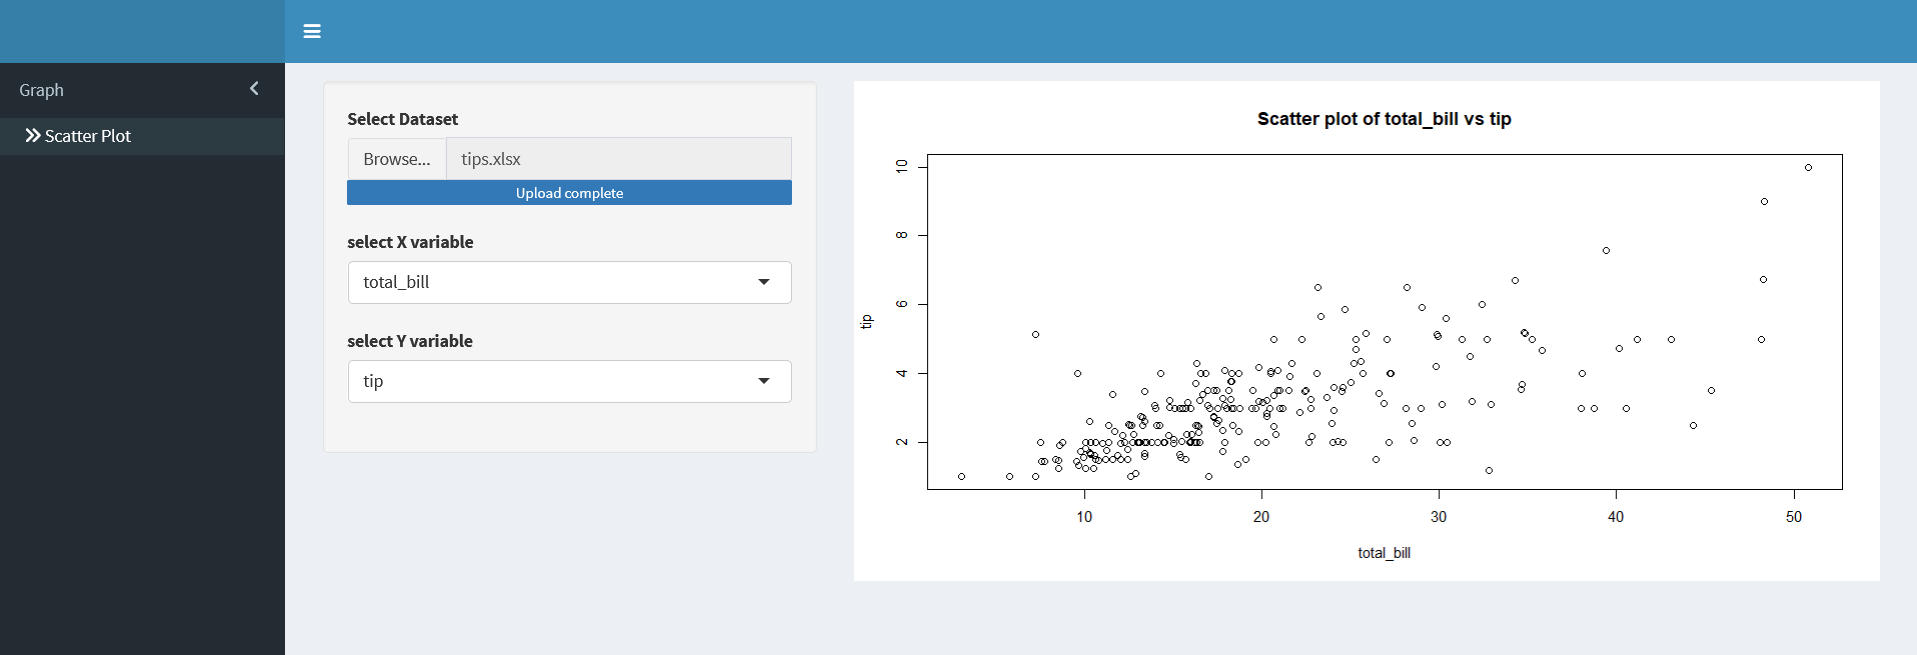
\includegraphics[width=0.8\textwidth,height=5.5cm]{scatter.png}
    \caption{scatter plot}
    \label{fig:image_label10}
   \end{figure}
\end{frame}


\begin{frame}{References}
    \begin{itemize}
    \item \href{https://shiny.rstudio.com/tutorial/written-tutorial/lesson1/}{Official Documentation}
    \item \href{https://www.youtube.com/watch?v=z5bUzdIbIyg&feature=youtu.be}{YouTube Channel}
    \item \href{https://stackoverflow.com/questions/40811903/in-shiny-update-datatable-with-new-values-from-user-input}{StackOverflow}
\end{itemize}
\vspace{1cm}
\begin{figure}[htbp]
    \centering
    
\includegraphics[width=0.7\textwidth,height=3cm]{thanks.png}
    % \caption{}
    \label{fig:image_label11}
   \end{figure}
\end{frame}


\end{document} 

